\section{Analisi}

In questa sezione verranno presentati e analizzati i risultati di benchmark.

Purtroppo, a causa di problemi tecnici con il cluster in dotazione, non è stato possibile valutare in maniera significativa gli algoritmi. In particolare, la funzione OpenMPI usata per creare la griglia di processi\footnote{\url{https://docs.open-mpi.org/en/v5.0.x/man-openmpi/man3/MPI_Cart_create.3.html}} potrebbe fallire arbitrariamente causando la chiusura forzata dell'eseguibile. Sperimentazioni ausiliarie hanno portato eventualmente sempre allo stesso errore, il che fa presagire possibili difetti nella versione della libreria installata.

È stato deciso di eseguire dei test locali su una singola macchina, ovviamente non indicativi delle prestazioni reali ma utili comunque a ricavare qualche spunto di riflessione.

\subsection{Configurazione dei test}

Per gestire l'esecuzione di un vasto numero di test con configurazioni eterogenee, sono stati implementati dei processi automatizzati tramite script.

\subsubsection{Locale}
Per eseguire i benchmark in locale, viene usato un semplice script che esegue sequenzialmente diversi test specificati, aggrega i risultati ottenuti e lancia uno script python per generare i grafici.
La macchina usata per eseguire i benchmark presenta:
\begin{itemize}
    \item CPU AMD Ryzen 5 7600;
    \item GPU NVIDIA GTX 1050Ti;
    \item 32 GB di RAM.
\end{itemize}

\subsubsection{Cluster}
Lanciare un'eseguibile sul cluster richiede maggiore pianificazione in quanto bisogna inviare una richiesta di \textit{job} tramite \textit{Slurm}, un sistema di gestione open source\footnote{\url{https://slurm.schedmd.com/overview.html}}. Lo script creato genera dinamicamente dei file batch a partire da configurazioni salvate in file di testo e richiede che vengano eseguiti. Nello specifico, si articola nelle seguenti fasi:

\begin{enumerate}
    \item \textbf{Inizializzazione} - viene preparato l'ambiente di esecuzione creando eventuali directory necessarie e rimuovendo i risultati di esecuzioni precedenti. Questo garantisce che ogni esecuzione parta da uno stato pulito e che i risultati non vengano contaminati da test precedenti.

    \item \textbf{Iterazione sui file di configurazione} - vengono letti tutti i file csv presenti nella directory \texttt{tests/}, ciascuno dei quali definisce una famiglia di test e specifica i parametri per una singola esecuzione.

    \item \textbf{Sottomissione dei job} - per ogni test da eseguire, lo script
          \begin{enumerate}
              \item esegue il parsing dei parametri (dimensioni della matrice, numero di processi, ...) estraendoli riga per riga;
              \item genera dinamicamente uno script di sottomissione Slurm contenente le direttive \texttt{\#SBATCH} necessarie per richiedere le risorse al cluster (nodi, GPU, file di output, ...);
              \item sottomette lo script creato al gestore di code tramite il comando \texttt{sbatch};
              \item aggiunge l'id del job a una lista di dipendenze che sarà utilizzata nella fase finale.
          \end{enumerate}

    \item \textbf{Job di analisi e plotting} - genera un ultimo job con una dipendenza di tipo \texttt{afterok} da tutti quelli sottomessi in precedenza, per eseguirlo solo dopo che tutti i test saranno terminati con successo. Il compito di questo job finale è aggregare i dati dei file csv generati ed eseguire uno script python per creare i grafici delle performance.
\end{enumerate}

\subsection{Analisi delle misurazioni}
Sono stati eseguiti i seguenti test:
\begin{enumerate}
    \item al crescere del numero di processi e threads, con dimensione fissata
          \begin{enumerate}
              \item al crescere delle dimensioni della matrice, a parità di processi (4) e thread (1024);
              \item al crescere del numero di processi, a parità di thread (1024) e dimensioni della matrice ($2048 \times 2048$);
              \item al crescere del numero di thread per processo, a parità di processi (4) e dimensioni della matrice ($2048 \times 2048$);
          \end{enumerate}
    \item al crescere del numero di processi, a parità di thread ($1024 \times 1024$) e dimensione del problema per processo ($1024 \times 1024$);
    \item al crescere del numero di thread, a parità di processi (4) e dimensione del problema per thread;
    \item al crescere del numero di processi, a parità di thread (1024) e dimensione del problema per thread.
\end{enumerate}

\begin{table}[H]
    \centering
    \begin{tabular}{cc}
        \hline
        \textbf{Matrice}    & \textbf{Tempo (s)} \\ \hline
        $16   \times 16   $ & 0.000012           \\
        $32   \times 32   $ & 0.000087           \\
        $64   \times 64   $ & 0.000573           \\
        $128  \times 128  $ & 0.004766           \\
        $256  \times 256  $ & 0.036135           \\
        $512  \times 512  $ & 0.284944           \\
        $1024 \times 1024 $ & 2.281789           \\
        $2048 \times 2048 $ & 18.509902          \\
        $4096 \times 4096 $ & 151.839314         \\ \hline
    \end{tabular}
    \caption{Tempi di esecuzione algoritmo sequenziale}
\end{table}

\begin{table}[H]
    \centering
    \begin{tabular}{cccccc}
        \hline
        \textbf{Matrice}   & \textbf{Processi} & \textbf{Thread} & \textbf{Tempo (s)} & \textbf{Speedup} & \textbf{Efficienza} \\
        \hline
        $32 \times 32$     & 4                 & 1024            & 0.111423           & 0.000646         & 0.000001            \\
        $64 \times 64$     & 4                 & 1024            & 0.111543           & 0.006562         & 0.000006            \\
        $128 \times 128$   & 4                 & 1024            & 0.107687           & 0.044731         & 0.000043            \\
        $256 \times 256$   & 4                 & 1024            & 0.112906           & 0.320620         & 0.000313            \\
        $512 \times 512$   & 4                 & 1024            & 0.151131           & 1.912400         & 0.001867            \\
        $1024 \times 1024$ & 4                 & 1024            & 0.403438           & 5.720774         & 0.005586            \\
        $2048 \times 2048$ & 4                 & 1024            & 2.104707           & 8.955829         & 0.008745            \\
        $4096 \times 4096$ & 4                 & 1024            & 16.102605          & 9.502196         & 0.009279            \\
        \hline
    \end{tabular}
    \caption{Metriche test 1a}
\end{table}

\begin{table}[H]
    \centering
    \begin{tabular}{cccccc}
        \hline
        \textbf{Matrice}   & \textbf{Processi} & \textbf{Thread} & \textbf{Tempo (s)} & \textbf{Speedup} & \textbf{Efficienza} \\
        \hline
        $2048 \times 2048$ & 2                 & 1024            & 2.149681           & 8.768461         & 0.008562            \\
        $2048 \times 2048$ & 4                 & 1024            & 2.112711           & 8.921899         & 0.008712            \\
        $2048 \times 2048$ & 8                 & 1024            & 2.233489           & 8.439439         & 0.008241            \\
        $2048 \times 2048$ & 16                & 1024            & 2.400357           & 7.852746         & 0.007668            \\
        \hline
    \end{tabular}
    \caption{Metriche test 1b}
\end{table}

\begin{table}[H]
    \centering
    \begin{tabular}{cccccc}
        \hline
        \textbf{Matrice}   & \textbf{Processi} & \textbf{Thread} & \textbf{Tempo (s)} & \textbf{Speedup} & \textbf{Efficienza} \\
        \hline
        $2048 \times 2048$ & 4                 & 16              & 86.549383          & 0.217787         & 0.013611            \\
        $2048 \times 2048$ & 4                 & 64              & 14.889047          & 1.265990         & 0.019781            \\
        $2048 \times 2048$ & 4                 & 256             & 3.294723           & 5.721086         & 0.022347            \\
        $2048 \times 2048$ & 4                 & 1024            & 2.115566           & 8.909859         & 0.008701            \\
        $2048 \times 2048$ & 4                 & 4096            & 0.634481           & 29.708369        & 0.007253            \\
        $2048 \times 2048$ & 4                 & 16384           & 0.487987           & 38.626840        & 0.002357            \\
        $2048 \times 2048$ & 4                 & 65536           & 0.457740           & 41.179263        & 0.000628            \\

        \hline
    \end{tabular}
    \caption{Metriche test 1c}
\end{table}

\begin{table}[H]
    \centering
    \begin{tabular}{cccccc}
        \hline
        \textbf{Matrice}   & \textbf{Processi} & \textbf{Thread} & \textbf{Tempo (s)} & \textbf{Speedup} & \textbf{Efficienza} \\
        \hline
        $1024 \times 1024$ & 1                 & 1024            & 0.315246           & 7.321196         & 0.007149            \\
        $2048 \times 2048$ & 4                 & 1024            & 2.124641           & 8.871802         & 0.008663            \\
        $4096 \times 4096$ & 16                & 1024            & 16.293719          & 9.390741         & 0.009170            \\
        \hline
    \end{tabular}
    \caption{Metriche test b}
\end{table}

\begin{table}[H]
    \centering
    \begin{tabular}{cccccc}
        \hline
        \textbf{Matrice}   & \textbf{Processi} & \textbf{Thread} & \textbf{Tempo (s)} & \textbf{Speedup} & \textbf{Efficienza} \\
        \hline
        $64 \times 64$     & 4                 & 16              & 0.107755           & 0.006793         & 0.000424            \\
        $128 \times 128$   & 4                 & 64              & 0.110345           & 0.043653         & 0.000682            \\
        $256 \times 256$   & 4                 & 256             & 0.113403           & 0.319215         & 0.001246            \\
        $512 \times 512$   & 4                 & 1024            & 0.144730           & 1.996980         & 0.001950            \\
        $1024 \times 1024$ & 4                 & 4096            & 0.191247           & 12.068048        & 0.002946            \\
        $2048 \times 2048$ & 4                 & 16384           & 0.507543           & 37.138520        & 0.002266            \\
        \hline
    \end{tabular}
    \caption{Metriche test c}
\end{table}

\begin{table}[H]
    \centering
    \begin{tabular}{cccccc}
        \hline
        \textbf{Matrice}   & \textbf{Processi} & \textbf{Thread} & \textbf{Tempo (s)} & \textbf{Speedup} & \textbf{Efficienza} \\
        \hline
        $1024 \times 1024$ & 1                 & 1024            & 0.311630           & 7.406148         & 0.007232            \\
        $2048 \times 2048$ & 4                 & 1024            & 2.121485           & 8.885000         & 0.008676            \\
        $4096 \times 4096$ & 16                & 1024            & 16.317378          & 9.377126         & 0.009157            \\
        \hline
    \end{tabular}
    \caption{Metriche test d}
\end{table}

\begin{figure}[ht]
    \centering
    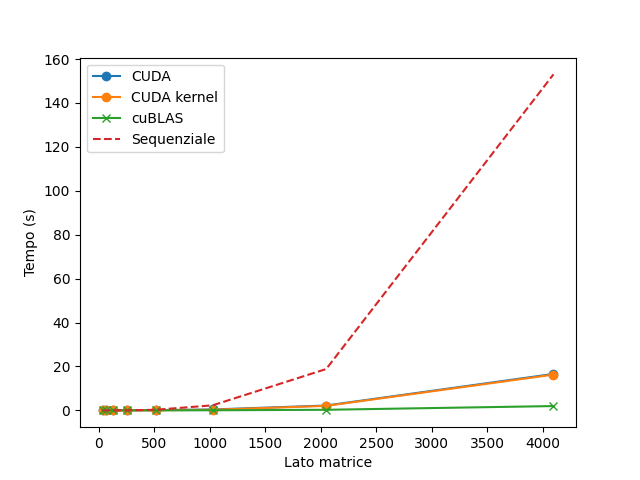
\includegraphics[width=0.7\textwidth]{./imgs/graphs/caso_0.png}
    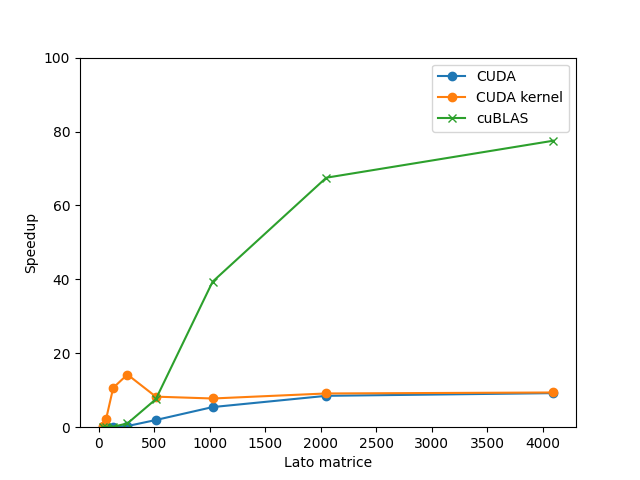
\includegraphics[width=0.7\textwidth]{./imgs/graphs/caso_0_speedup.png}
    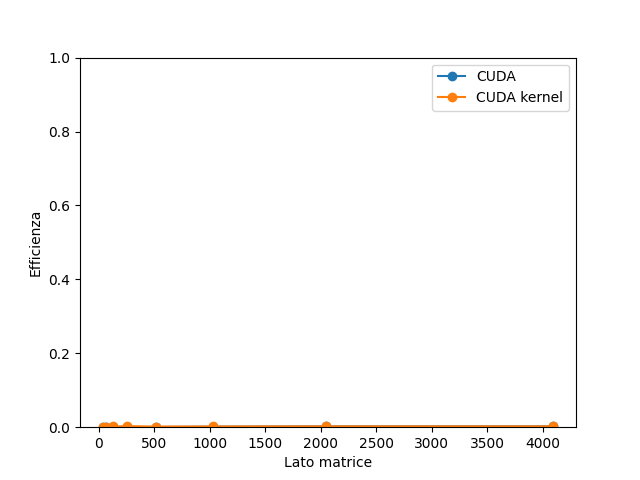
\includegraphics[width=0.7\textwidth]{./imgs/graphs/caso_0_efficiency.png}
    \caption{Caso 1a}
\end{figure}

\begin{figure}[ht]
    \centering
    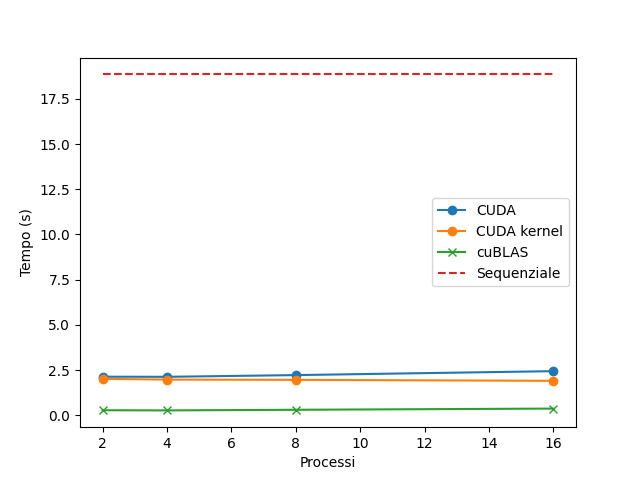
\includegraphics[width=0.7\textwidth]{./imgs/graphs/caso_a1.png}
    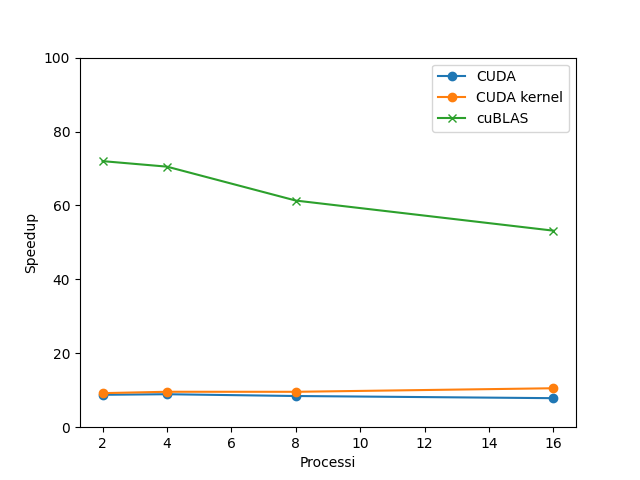
\includegraphics[width=0.7\textwidth]{./imgs/graphs/caso_a1_speedup.png}
    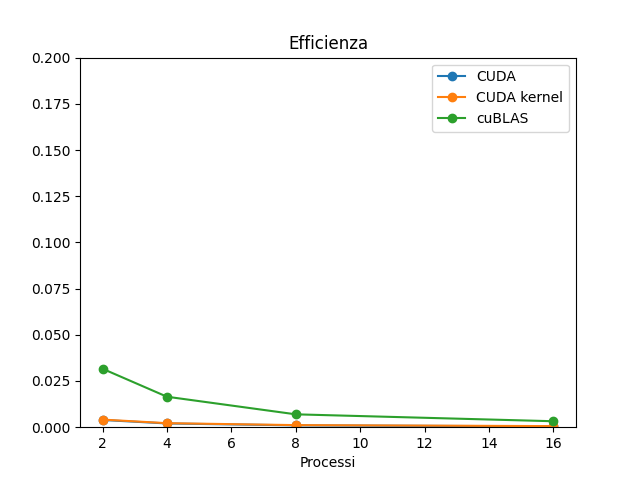
\includegraphics[width=0.7\textwidth]{./imgs/graphs/caso_a1_efficiency.png}
    \caption{Caso 1b}
\end{figure}

\begin{figure}[ht]
    \centering
    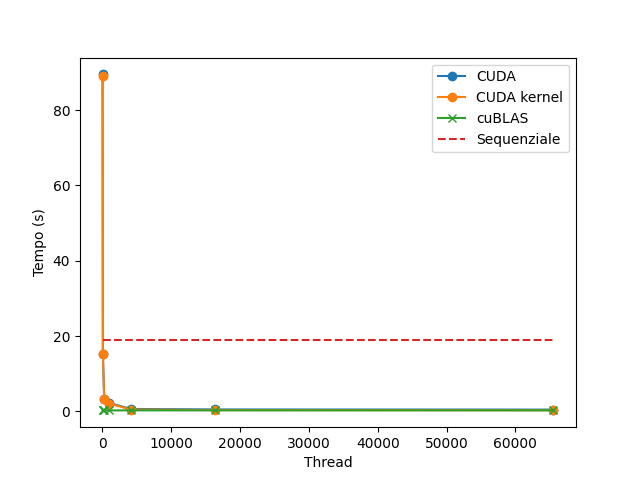
\includegraphics[width=0.7\textwidth]{./imgs/graphs/caso_a2.png}
    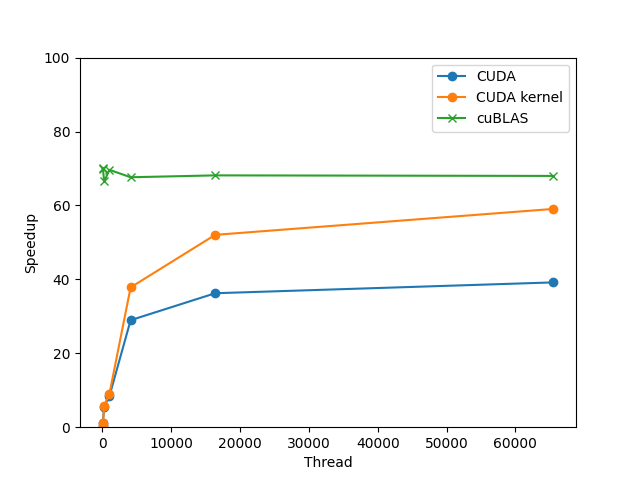
\includegraphics[width=0.7\textwidth]{./imgs/graphs/caso_a2_speedup.png}
    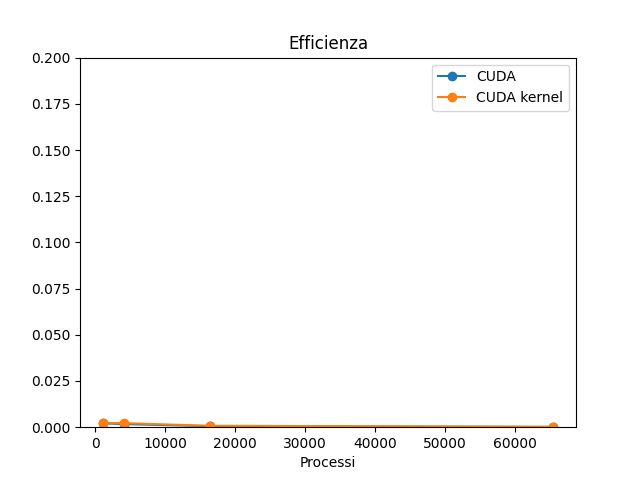
\includegraphics[width=0.7\textwidth]{./imgs/graphs/caso_a2_efficiency.png}
    \caption{Caso 1c}
\end{figure}

\begin{figure}[ht]
    \centering
    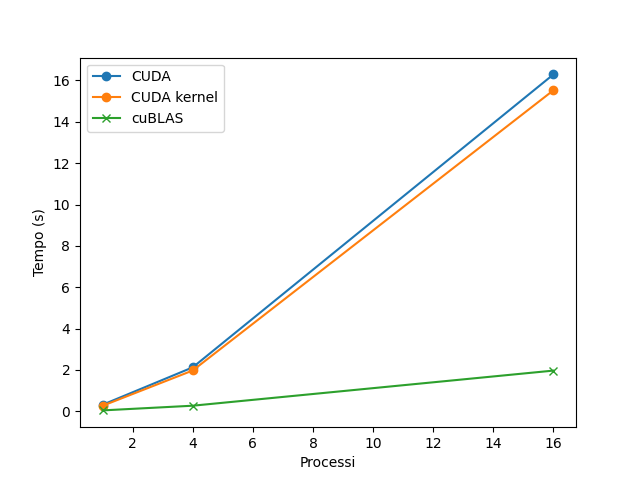
\includegraphics[width=0.7\textwidth]{./imgs/graphs/caso_b.png}
    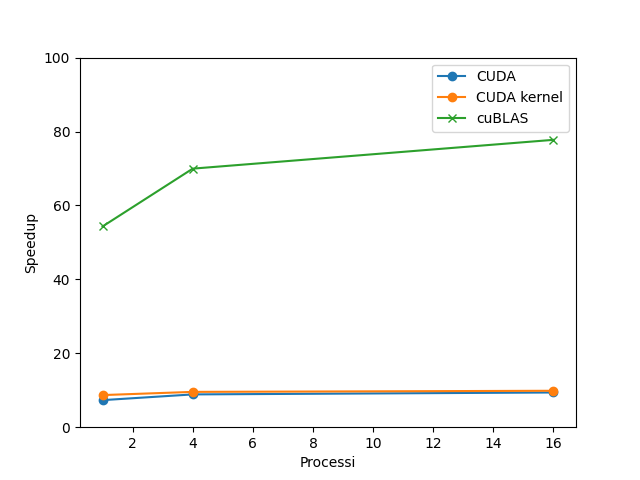
\includegraphics[width=0.7\textwidth]{./imgs/graphs/caso_b_speedup.png}
    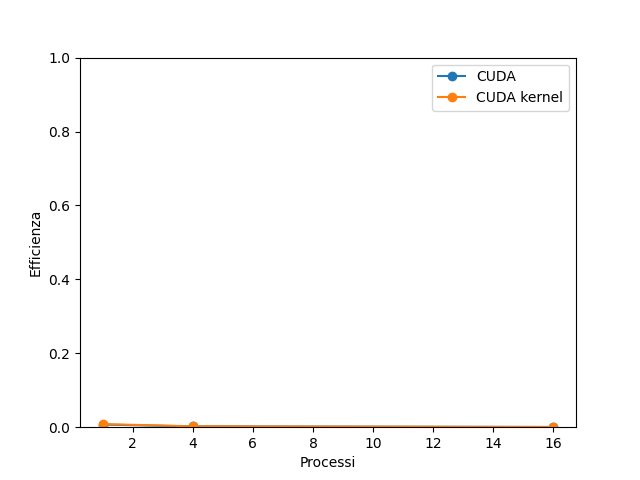
\includegraphics[width=0.7\textwidth]{./imgs/graphs/caso_b_efficiency.png}
    \caption{Caso 2}
\end{figure}

\begin{figure}[ht]
    \centering
    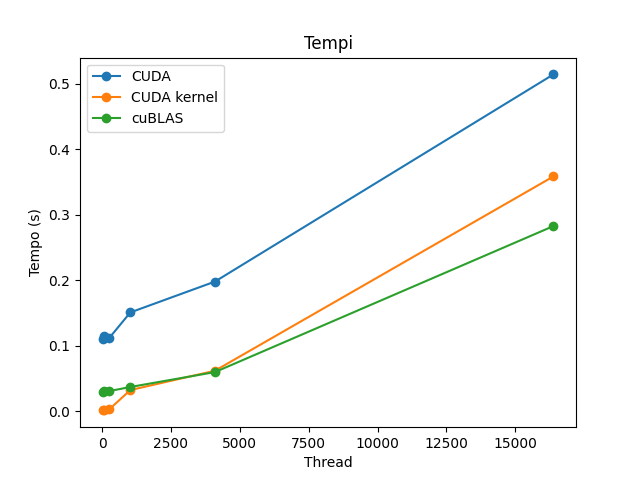
\includegraphics[width=0.7\textwidth]{./imgs/graphs/caso_c.png}
    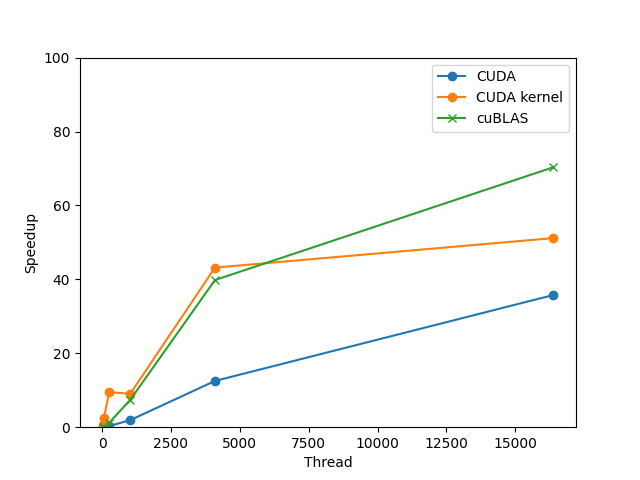
\includegraphics[width=0.7\textwidth]{./imgs/graphs/caso_c_speedup.png}
    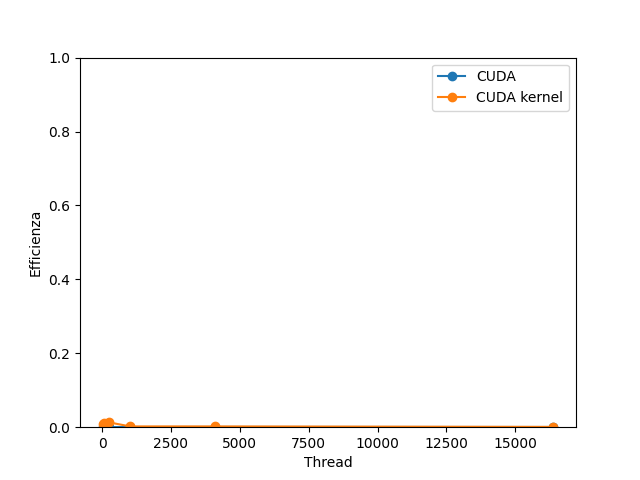
\includegraphics[width=0.7\textwidth]{./imgs/graphs/caso_c_efficiency.png}
    \caption{Caso 3}
\end{figure}

\begin{figure}[ht]
    \centering
    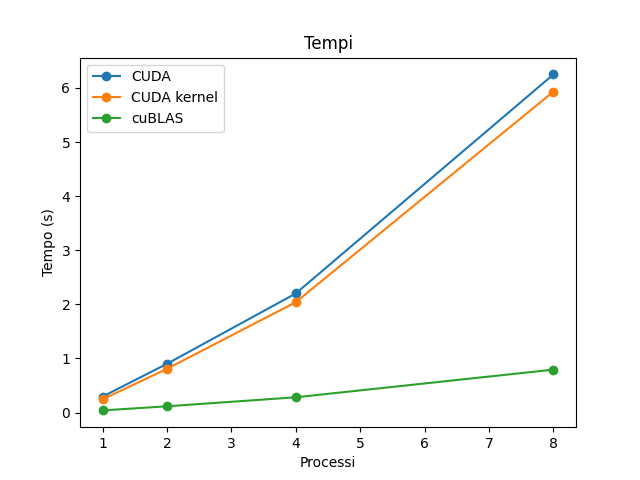
\includegraphics[width=0.7\textwidth]{./imgs/graphs/caso_d.png}
    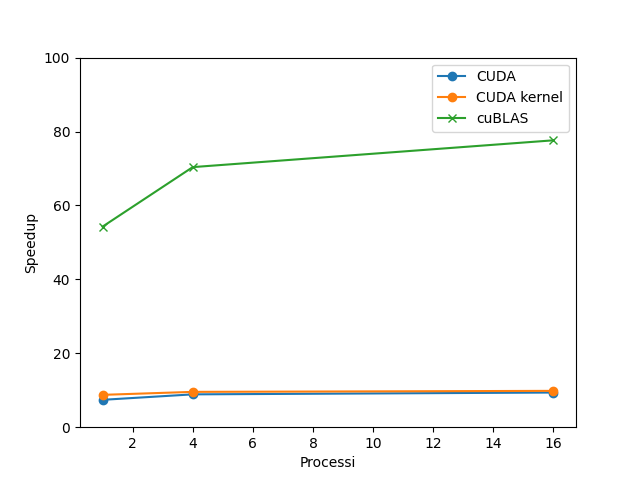
\includegraphics[width=0.7\textwidth]{./imgs/graphs/caso_d_speedup.png}
    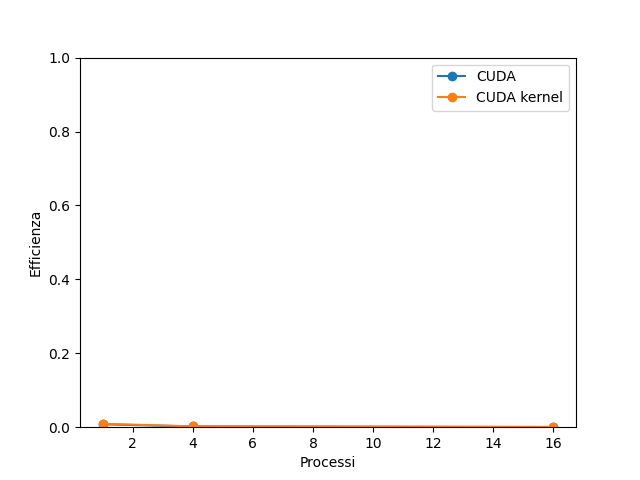
\includegraphics[width=0.7\textwidth]{./imgs/graphs/caso_d_efficiency.png}
    \caption{Caso 4}
\end{figure}

Non è possibile trarre conclusioni certe date le limitazioni del caso, ma è possibile notare come non convenga usare le GPU per per matrici di piccole dimensioni\footnote{$\approx 512 \times 512$} dato che l'overhead causa tempi di esecuzione maggiori rispetto a quelli dell'algoritmo sequenziale.

Dai tempi di esecuzione e dallo speedup ottenuto nei vari casi, conviene aumentare il numero di thread piuttosto che distribuire il carico aumentando i processi. Ciò probabilmente è dovuto al fatto che i processi non riescono a utilizzare tutti contemporaneamente la GPU causando delle attese.

In questo caso, i trasferimenti di memoria non rappresentano più di tanto un collo di bottiglia ma l'utilizzo concorrente della stessa GPU da parte di più processi causa ovviamente dei tempi di attesa.

Un risultato leggermente preoccupante è l'efficienza praticamente nulla ottenuta dai vari test. Ciò può risultare sia dalle condizioni dei benchmark effettuati che dal numero estremamente grande di thread utilizzati.

\subsection{NVIDIA Nsight Compute}

Nsight Compute è uno strumento di profilazione delle prestazioni delle GPU sviluppato da NVIDIA, pensato specificamente per analizzare ed ottimizzare i kernel CUDA. Fornisce un'analisi dettagliata del comportamento del codice sulla GPU, consentendo di identificare colli di bottiglia come utilizzo inefficiente della memoria (global, shared, cache), occupancy bassa dei multiprocessori, warp divergence, stalli nelle pipeline di esecuzione. È altamente configurabile, supporta analisi interattive via GUI o in modalità batch da riga di comando, e consente di confrontare facilmente più esecuzioni.

Purtroppo, a causa dei problemi tecnici riportati precedentemente, non è stato possibile valutare le metriche fornite da queste applicazioni.
